%! Author = Tom
%! Date = 07.12.2022
\section{Einleitung}

In diesem Kapitel wird an das Thema und die Motivation dieser Arbeit herangeführt.
Außerdem wird definiert, welche Ziele diese Arbeit erreichen soll und eine grobe Übersicht über die
Kapitelstruktur gegeben.

\subsection{Motivation}

Mit einer steigenden Nutzung von GraphQL wird es immer wichtiger, geeignete Tests für GraphQL-API's zu entwickeln damit eine
gute Softwarequalität sichergestellt werden kann. Idealerweise können diese Testtools solche API's automatisch testen,
so wie es für REST-API's schon umgesetzt wurde. Die Struktur von GraphQL erlaubt allerdings zyklische Strukturen
und ermöglicht somit ein potentenziell undendlich großen Testraum.
In einem Paper "Automatic Property-based Testing of GraphQL-API's" (hier Quelle) wurde versucht ein solches
automatisches Testtool schon umzusetzen. Allerdings hat dieses Paper zwei große Verbesserungspunkte. 
Einerseits die Art, wie die Tests generiert werden, andererseits die Auswertung der Tests.
Der allgemeine Ablauf des bestehenden Tools ist wie folgt:

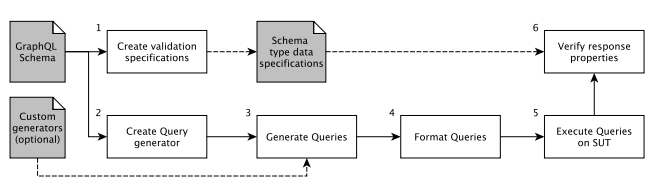
\includegraphics{content/einleitung/toolchain}

Verbesserungen in dieser Arbeit sind insbesondere in den Punkten 2,3 und 6 geplant.

\begin{description}
    \item[Create Query Generator (Punkt 2)] Kapitel Testgenerierung
    \item[Generate Queries (Punkt 3)]  Kapitel Testgenerierung
    \item[Verify response properties (Punkt 6)] Kapitel Testauswertung
\end{description}



\subsubsection*{Testgenerierung}

Bei der Testgenerierung wurde mit den zyklischen Strukturen in GraphQL Schemas so
umgegangen, dass eine Rekursionstiefe definiert wurde, damit man das Problem des unendlichen Testraumes beheben kann.
Dieser Ansatz erlaubt es aber leider nicht, dass eine ideale Abdeckung (was das ist wird später genau
definiert) gewährleistet werden kann.
Insbesondere komplexere, zyklische Strukturen werden hierbei von dem automatischen
Tool nicht getestet da die Rekursionstiefe dies oft nicht erlaubt.
Mit der Nutzung von graphspezifischen Algorithmen ist es jedoch möglich Graphabdeckungen zu ermitteln auch wenn diese
eine zyklische Struktur haben und somit kann algoritmisch das Problem des Papers gelöst werden.
In dieser Arbeit sollen diese graphspezifischen Algorithmen implementiert werden und dann mittels Datengeneratoren eigenständig
Tests erzeugen.

\subsubsection*{Testauswertung}

Die Auswertung der Tests ist im Paper darauf basierend, dass die zu testende API vor allem auch funktionale Korrektheit überprüft wird,
dies bedeutet insbesondere, dass hier die HTTP-Status Codes von Anfragen ausgewertet werden sowie GraphQL eigene Statusmeldungen untersucht werden.
Ein richtiger Abgleich im Test findet nicht statt, es wird lediglich überprüft ob der Rückgabe-Datentyp dem erwarteten Datentyp entspricht.
Es wäre jedoch besser wenn nicht nur der Rückgabe-Datentyp stimmt sondern auch der Inhalt in diesem Datentyp. In dieser Arbeit
soll das Programm mittels eines Orakels verbessert werden. Dies bedeutet, dass die GraphQL API mit Testdaten befüllt wird und Anfragen
gestellt werden können, die sich dann auch logisch ineinander auflösen. Hierbei ist insbesondere zu beachten, dass Kreisstrukturen sich in gewisser Weise
in sich selbst auflösen, d.h. Eingabeobjekt = Ausgabeobjekt.

\subsection{Umsetzung}

Zuallererst wird in dieser Arbeit etwas Theorie definiert und in Bezug gesetzt. Angefangen mit einer allgemeinen Definition
eines Graphens im mathematischen Sinne und GraphQL als Schnittstelle, wird dann ein Bezug dieser beiden Themen
zueinander hergestellt. Wenn der Bezug von Graphentheorie und GraphQL klar ist, wird der eigentliche Algorithmus für die
ideale Abdeckung des Graphens algorithmisch erklärt, eine Anwendung auf GraphQL in der Theorie gezeigt und bewiesen.
Danach werden die theoretischen Erkenntnisse in einem praktischen Projekt umgesetzt. Hierbei wird ein Tool erstellt,
welches aufgrundlage des Überdeckungsalgorithmus & einem Datengenerator Tests erstellt und dann auswertet mittels
den alten bzw. erweiterten Ablgeichsmethoden. Um zu zeigen, dass das neue Verfahren eine Verbesserung darstellt wird dann
ein Benchmark Test zwischen altem und neuen System erstellt. Bei diesem Benchmark Test werden 3 verschiedene
GraphQL-Schemas getestet, 2 Schemas aus dem alten Paper, hier ergibt sich ein direkter Vergleich an z.B. generierten Tests und
Graphabdeckung. Im 3ten Schema wird ein speziell sehr zyklisches Schema ausgewertet um zu zeigen, dass einerseits die Implementierung
den Algorithmus korrekt umsetzt und wie groß die Verbesserung in solchen Schemas dann sind.
